% Generated by docs-notes/figures/build-figures.mjs. Do not edit by hand:
% edit the TikZ in docs-notes/FIGURES.md and re-run the script.
\documentclass[11pt,a4paper]{article}
\usepackage[T1]{fontenc}
\usepackage[utf8]{inputenc}
\usepackage{lmodern}
\usepackage{booktabs}
\usepackage{textcomp}
\usepackage{graphicx}
\usepackage[margin=20mm]{geometry}
\usepackage{tikz}
\usetikzlibrary{arrows.meta, positioning, shapes.geometric, fit, backgrounds, calc,
                decorations.pathreplacing}
\usepackage{pgfplots}
\pgfplotsset{compat=1.18}
\tikzset{
  gbox/.style   = {draw=black!55, fill=black!3, rounded corners=2pt,
                   align=center, font=\small, inner sep=5pt, minimum height=9mm},
  gnote/.style  = {draw=none, fill=none, align=center, font=\scriptsize\itshape},
  gdec/.style   = {draw=black!55, fill=black!8, diamond, aspect=2.2,
                   align=center, font=\scriptsize, inner sep=1pt},
  gstore/.style = {draw=black!55, fill=black!6, align=center,
                   font=\scriptsize, inner sep=5pt},
  ggroup/.style = {draw=black!35, dashed, rounded corners=3pt, inner sep=7pt},
  gflow/.style  = {-{Stealth[length=2mm]}, draw=black!70},
  gdash/.style  = {-{Stealth[length=2mm]}, draw=black!70, dashed},
  glab/.style   = {font=\scriptsize, fill=white, inner sep=1.5pt},
  glife/.style  = {draw=black!45, dashed}
}
\begin{document}
\begin{center}\Large\textbf{Governance layer: report figures}\\[2pt]
\normalsize Extracted from \texttt{docs-notes/FIGURES.md} for T17 approval.\end{center}
\vspace{4mm}
\section*{Chapter 3}
\subsection*{Figure 3.1 \textnormal{(F1: Governance layer within the OpenClaw Gateway)}}
\begin{center}
\begin{figure}[htbp]
\centering
  % Measured too wide for the text block when compiled (2026-09-20), so it is
  % scaled to the text width rather than having its font sizes changed.
\resizebox{\textwidth}{!}{%
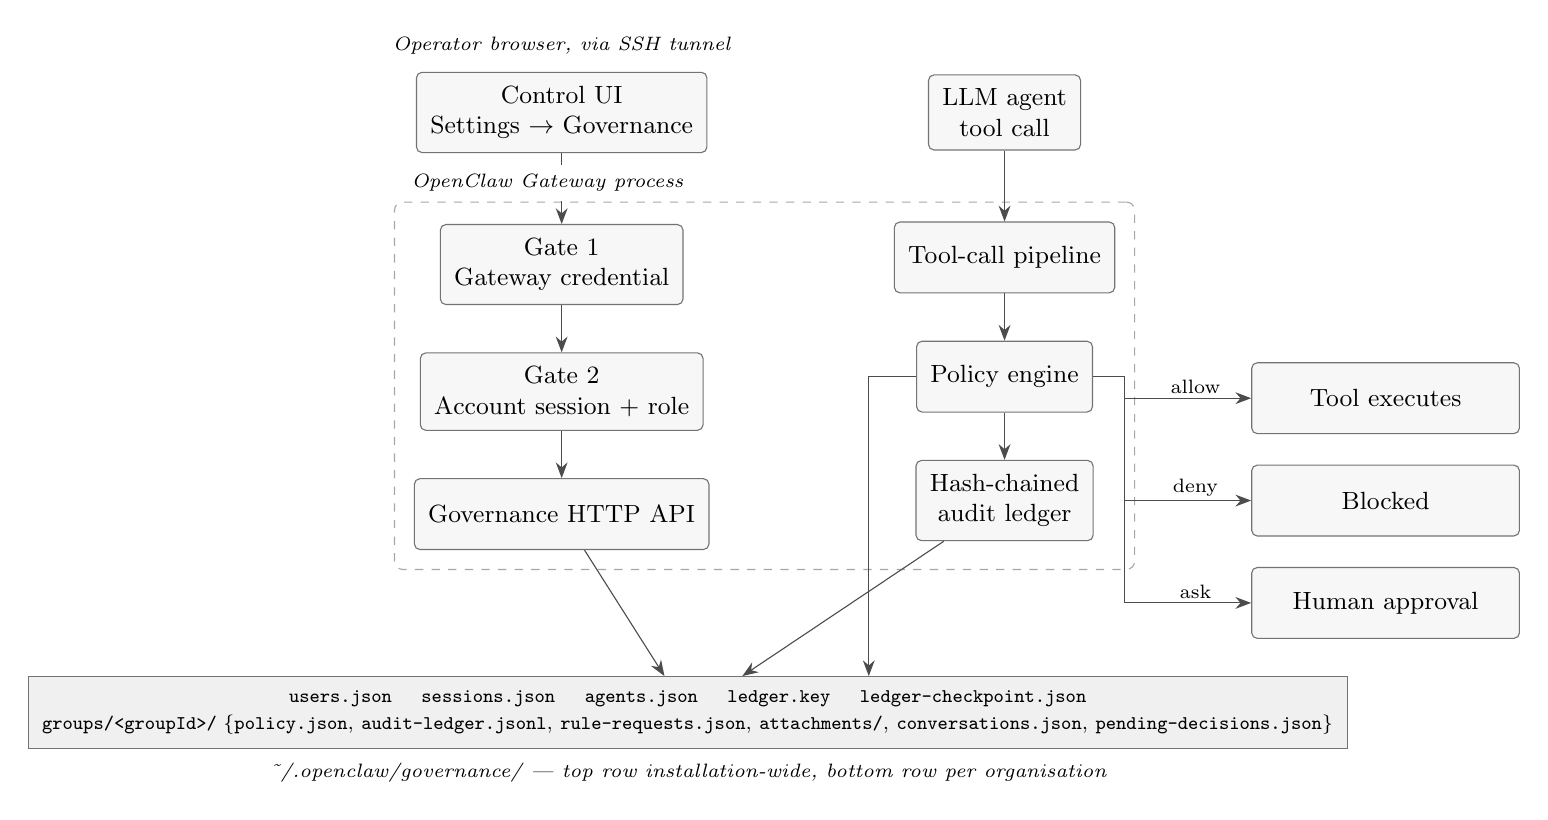
\begin{tikzpicture}[node distance=6mm and 10mm]
  \node[gbox] (ui) {Control UI\\Settings $\rightarrow$ Governance};
  \node[gnote, above=1mm of ui] {Operator browser, via SSH tunnel};

  \node[gbox, below=9mm of ui] (auth) {Gate 1\\Gateway credential};
  \node[gbox, below=of auth]   (rbac) {Gate 2\\Account session + role};
  \node[gbox, below=of rbac]   (api)  {Governance HTTP API};

  \node[gbox, right=28mm of ui]   (agent)  {LLM agent\\tool call};
  \node[gbox, below=9mm of agent] (pipe)   {Tool-call pipeline};
  \node[gbox, below=of pipe]      (engine) {Policy engine};
  \node[gbox, below=of engine]    (ledger) {Hash-chained\\audit ledger};

  \node[gstore, below=16mm of api, xshift=16mm] (disk)
    {\texttt{users.json} \quad \texttt{sessions.json} \quad \texttt{agents.json}
     \quad \texttt{ledger.key} \quad \texttt{ledger-checkpoint.json}\\[2pt]
     \texttt{groups/<groupId>/}\;\{\texttt{policy.json},
     \texttt{audit-ledger.jsonl}, \texttt{rule-requests.json}, \texttt{attachments/},
     \texttt{conversations.json}, \texttt{pending-decisions.json}\}};
  \node[gnote, below=0.5mm of disk]
    {\textasciitilde/.openclaw/governance/ --- top row installation-wide, bottom row per organisation};

  % 13mm apart, not 9: a gbox is 9mm tall, so 9mm of shift stacks them edge to edge.
  % One minimum width so the three outcomes read as one set.
  \node[gbox, minimum width=34mm, right=20mm of ledger, yshift=13mm]  (allow) {Tool executes};
  \node[gbox, minimum width=34mm, right=20mm of ledger]               (deny)  {Blocked};
  \node[gbox, minimum width=34mm, right=20mm of ledger, yshift=-13mm] (ask)   {Human approval};

  \draw[gflow] (ui)     -- (auth);
  \draw[gflow] (auth)   -- (rbac);
  \draw[gflow] (rbac)   -- (api);
  \draw[gflow] (agent)  -- (pipe);
  \draw[gflow] (pipe)   -- (engine);
  \draw[gflow] (engine) -- (ledger);
  \draw[gflow] (api)    -- (disk);
  \draw[gflow] (ledger) -- (disk);
  % Straight down onto the store's top edge. "|- (disk.west)" ran the line through
  % the store and out of its left side, across the text (found by looking, 2026-09-20).
  \coordinate (enginedrop) at ([xshift=-6mm]engine.west);
  \draw[gflow] (engine.west) -- (enginedrop) -- (enginedrop |- disk.north);

  % Labels sit above the horizontal run: a glab is filled white, and on the run
  % itself it painted over the arrow head it was meant to name.
  \draw[gflow] (engine.east) -- ++(4mm,0) |- node[glab, above, pos=0.78] {allow} (allow.west);
  \draw[gflow] (engine.east) -- ++(4mm,0) |- node[glab, above, pos=0.78] {deny}  (deny.west);
  \draw[gflow] (engine.east) -- ++(4mm,0) |- node[glab, above, pos=0.78] {ask}   (ask.west);

  \begin{scope}[on background layer]
    \node[ggroup, fit=(auth)(rbac)(api)(pipe)(engine)(ledger)] (gw) {};
  \end{scope}
  % Above the dashed border, not inside it: anchored north west the label sat on
  % top of the Gate 1 box (found by looking, 2026-09-20).
  \node[gnote, fill=white, anchor=south west, xshift=1mm] at (gw.north west) {OpenClaw Gateway process};
\end{tikzpicture}}
\caption{Governance layer within the OpenClaw Gateway.}
\label{fig:architecture}
\end{figure}
\end{center}
\clearpage
\subsection*{Figure 3.2 \textnormal{(F2: RBAC hierarchy with inherited permissions)}}
\begin{center}
\begin{figure}[htbp]
\centering
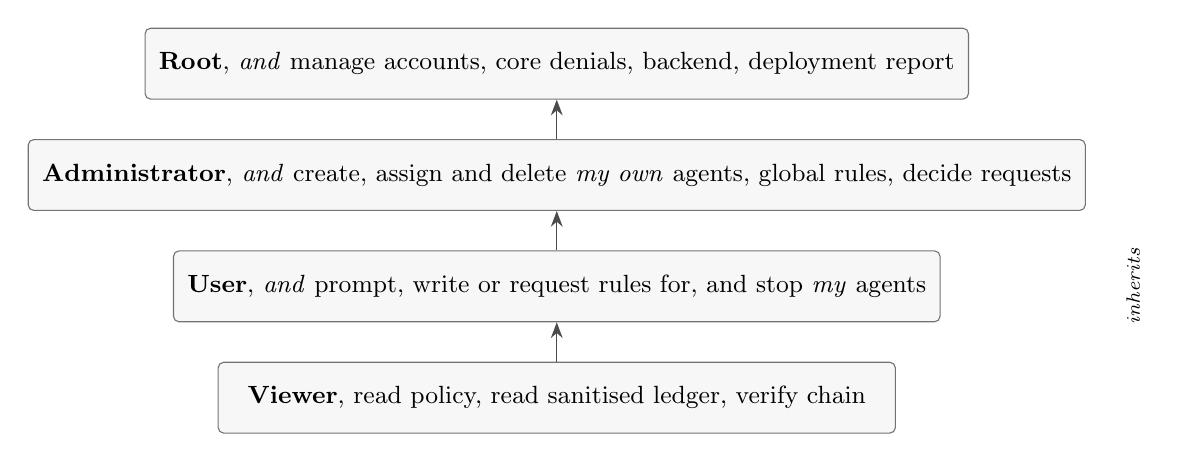
\begin{tikzpicture}[node distance=5mm]
  \node[gbox, minimum width=86mm] (v) {\textbf{Viewer}, read policy, read sanitised ledger, verify chain};
  \node[gbox, minimum width=86mm, above=of v] (u) {\textbf{User}, \textit{and} prompt, write or request rules for, and stop \emph{my} agents};
  \node[gbox, minimum width=86mm, above=of u] (a) {\textbf{Administrator}, \textit{and} create, assign and delete \emph{my own} agents, global rules, decide requests};
  \node[gbox, minimum width=86mm, above=of a] (r) {\textbf{Root}, \textit{and} manage accounts, core denials, backend, deployment report};
  \draw[gflow] (v) -- (u);
  \draw[gflow] (u) -- (a);
  \draw[gflow] (a) -- (r);
  % Beside the stack and clear of it. "right=3mm of u" measured off the User row,
  % which is narrower than the Administrator row, so the label landed on top of the
  % boxes (found by looking, 2026-09-20).
  \node[gnote, rotate=90] at ([xshift=6mm]a.east |- u) {inherits};
\end{tikzpicture}
\caption{Role hierarchy. Each tier inherits every capability below it. The emergency stop sits at \textbf{User}, scoped to the agents assigned to that account, not at Root. An Administrator acts on one agent only when it owns that agent; Root may act on any.}
\label{fig:rbac}
\end{figure}
\end{center}
\clearpage
\subsection*{Figure 3.3 \textnormal{(F3: Policy decision sequence)}}
\begin{center}
\begin{figure}[htbp]
\centering
  % Measured too wide for the text block when compiled (2026-09-20), so it is
  % scaled to the text width rather than having its font sizes changed.
\resizebox{\textwidth}{!}{%
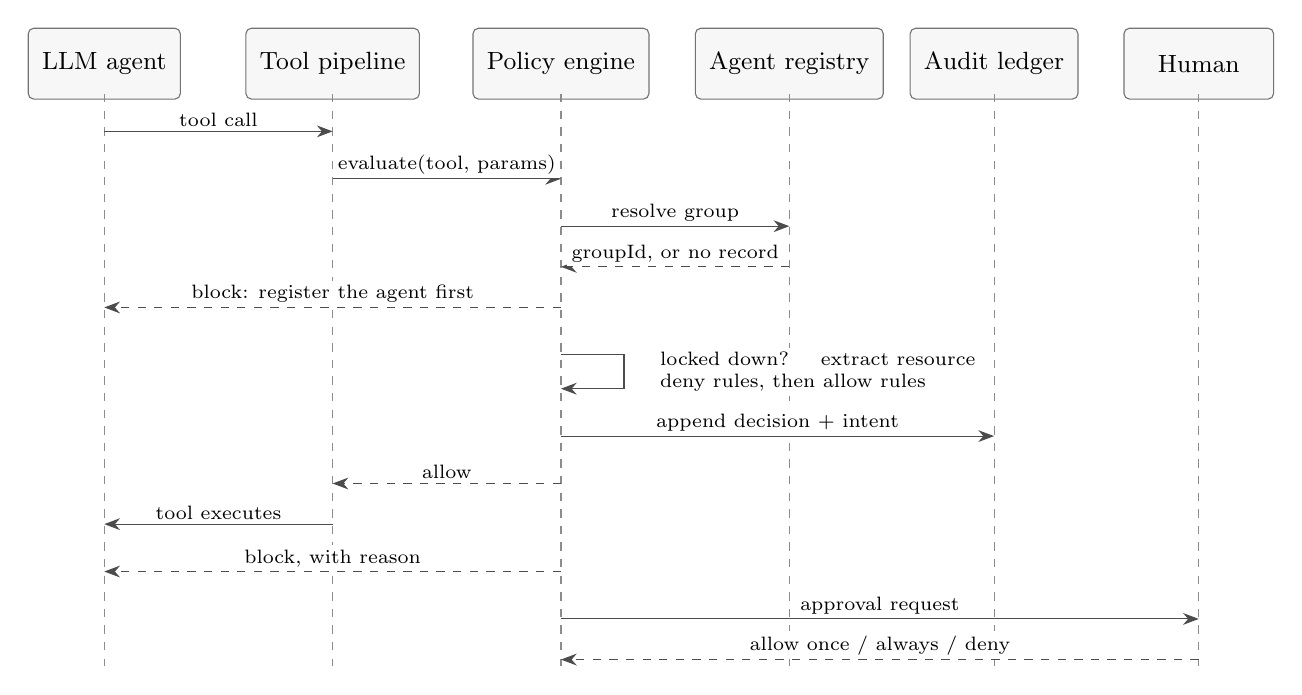
\begin{tikzpicture}[yscale=0.86]
  \foreach \x/\n in {0/{LLM agent}, 2.9/{Tool pipeline}, 5.8/{Policy engine},
                     8.7/{Agent registry}, 11.3/{Audit ledger}, 13.9/{Human}} {
    \node[gbox, minimum width=19mm] at (\x,0) {\n};
    \draw[glife] (\x,-0.45) -- (\x,-8.9);
  }
  \draw[gflow] (0,-1.0)   -- node[glab,above] {tool call} (2.9,-1.0);
  \draw[gflow] (2.9,-1.7) -- node[glab,above] {evaluate(tool, params)} (5.8,-1.7);

  \draw[gflow] (5.8,-2.4) -- node[glab,above] {resolve group} (8.7,-2.4);
  \draw[gdash] (8.7,-3.0) -- node[glab,above] {groupId, or no record} (5.8,-3.0);
  \draw[gdash] (5.8,-3.6) -- node[glab,above] {block: register the agent first} (0,-3.6);

  \draw[gflow] (5.8,-4.3) -- ++(0.8,0) -- ++(0,-0.5) -- (5.8,-4.8);
  % Off a declared coordinate: "of {(x,y)}" drops its own closing bracket
  % into nullfont (found by compiling, 2026-09-20).
  \coordinate (selfloop) at (5.8,-4.55);
  % Close to the loop and on two lines. At 32mm out and on one line it ran past the
  % last lifeline and off the figure (found by looking, 2026-09-20); glab is filled,
  % so the lifelines it does cross stay out of the words.
  \node[glab, right=12mm of selfloop, align=left]
    {locked down? \quad extract resource\\deny rules, then allow rules};

  \draw[gflow] (5.8,-5.5) -- node[glab,above] {append decision + intent} (11.3,-5.5);

  \draw[gdash] (5.8,-6.2) -- node[glab,above] {allow} (2.9,-6.2);
  \draw[gflow] (2.9,-6.8) -- node[glab,above] {tool executes} (0,-6.8);
  \draw[gdash] (5.8,-7.5) -- node[glab,above] {block, with reason} (0,-7.5);

  \draw[gflow] (5.8,-8.2) -- node[glab,above] {approval request} (13.9,-8.2);
  \draw[gdash] (13.9,-8.8) -- node[glab,above] {allow once / always / deny} (5.8,-8.8);
\end{tikzpicture}}
\caption{Policy decision sequence, in the shipped \texttt{enforce} posture (under
\texttt{monitor} a call no allow rule covers is recorded and then allowed; under
\texttt{off} the gate records nothing). An unregistered agent is refused before any
policy is read. Deny rules are checked before allow rules, so a matching denial
refuses the call whatever any allowance says, even in monitor posture. Of the
remaining paths, the first is taken when an allow rule matches and the other two
when none does, depending on whether escalation is enabled. The human who answers
is, for a dashboard prompt, an account that manages the agent, and for a chat run,
whoever holds the Gateway credential. An ``allow always'' answer permits that one
call and files a rule request for an administrator to approve; it does not write a
rule by itself.}
\label{fig:decision}
\end{figure}
\end{center}
\clearpage
\subsection*{Figure 3.4 \textnormal{(F5: Path normalisation pipeline)}}
\begin{center}
\begin{figure}[htbp]
\centering
\resizebox{\textwidth}{!}{%
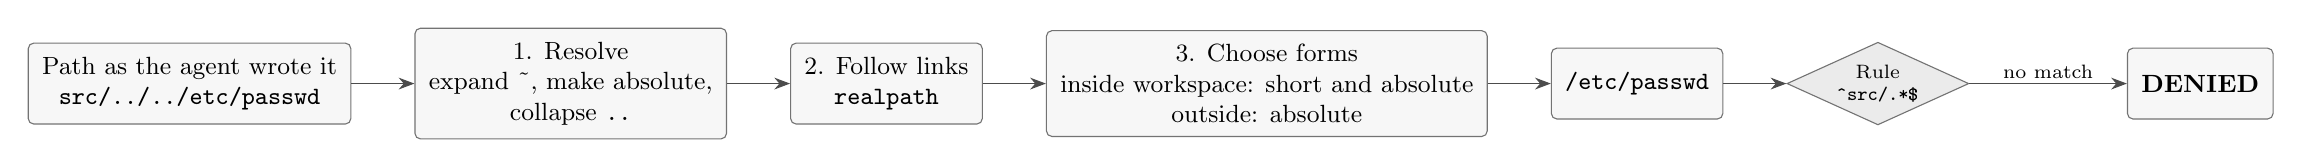
\begin{tikzpicture}[node distance=8mm]
  \node[gbox] (raw) {Path as the agent wrote it\\\texttt{src/../../etc/passwd}};
  \node[gbox, right=of raw] (s1) {1. Resolve\\expand \textasciitilde, make absolute,\\collapse \texttt{..}};
  \node[gbox, right=of s1]  (s2) {2. Follow links\\\texttt{realpath}};
  \node[gbox, right=of s2]  (s3) {3. Choose forms\\inside workspace: short and absolute\\outside: absolute};
  \node[gbox, right=of s3]  (out) {\texttt{/etc/passwd}};
  \node[gdec, right=of out] (rule) {Rule\\\texttt{\^{}src/.*\$}};
  % 20mm, not the default 8: "no match" is wider than the gap and sat on the box
  % (found by looking, 2026-09-20).
  \node[gbox, right=20mm of rule] (deny) {\textbf{DENIED}};

  \draw[gflow] (raw) -- (s1);
  \draw[gflow] (s1)  -- (s2);
  \draw[gflow] (s2)  -- (s3);
  \draw[gflow] (s3)  -- (out);
  \draw[gflow] (out) -- (rule);
  \draw[gflow] (rule) -- node[glab, above] {no match} (deny);
\end{tikzpicture}}
\caption{Path normalisation. The rule is matched against what the path resolves
to, not against what the agent typed; a path inside the workspace is matched in
both its short and its absolute form.}
\label{fig:pathnorm}
\end{figure}
\end{center}
\clearpage
\subsection*{Figure 3.5 \textnormal{(F6: The governed prompt path)}}
\begin{center}
\begin{figure}[htbp]
\centering
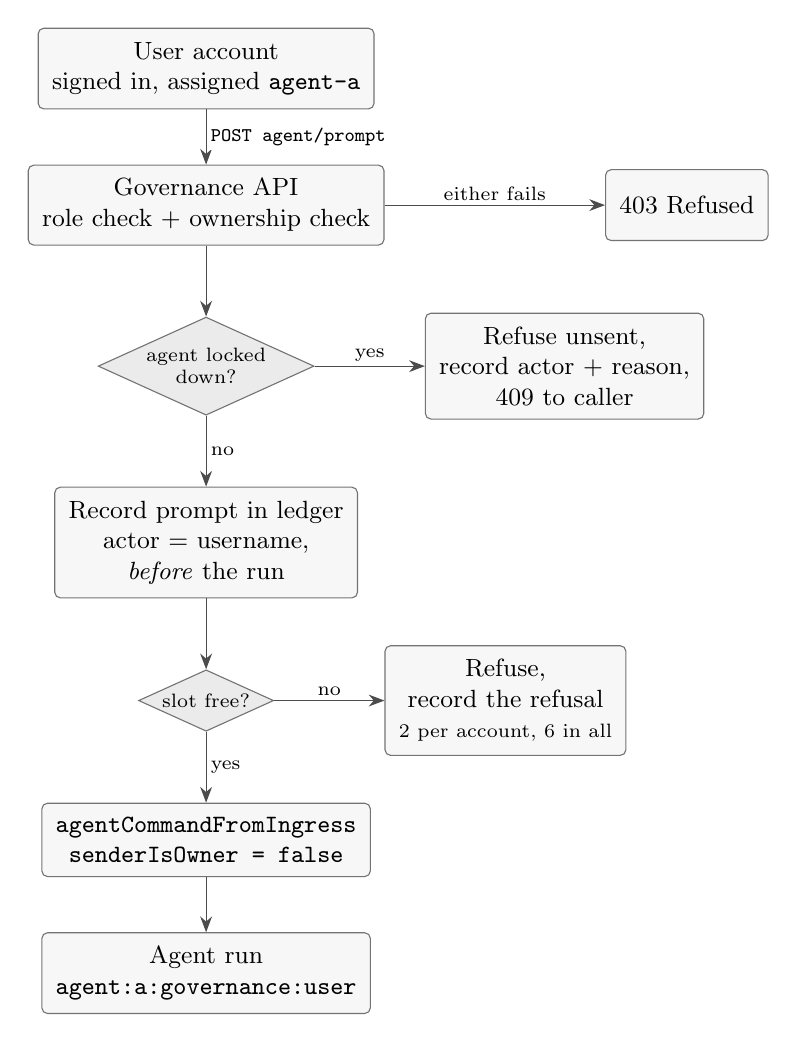
\begin{tikzpicture}[node distance=7mm and 14mm]
  \node[gbox] (u) {User account\\signed in, assigned \texttt{agent-a}};
  \node[gbox, below=of u]   (api)  {Governance API\\role check + ownership check};
  \node[gdec, below=9mm of api] (lock) {agent locked\\down?};
  \node[gbox, below=9mm of lock] (rec) {Record prompt in ledger\\actor = username,\\\textit{before} the run};
  \node[gdec, below=9mm of rec] (slot) {slot free?};
  \node[gbox, below=9mm of slot] (ing) {\texttt{agentCommandFromIngress}\\\texttt{senderIsOwner = false}};
  \node[gbox, below=of ing] (run) {Agent run\\\texttt{agent:a:governance:user}};

  % 28mm, not the default 14: "either fails" is wider than the gap and sat on the
  % box (found by looking, 2026-09-20).
  \node[gbox, right=28mm of api]  (deny) {403 Refused};
  \node[gbox, right=of lock] (ref)  {Refuse unsent,\\record actor + reason,\\409 to caller};
  \node[gbox, right=of slot] (full) {Refuse,\\record the refusal\\\scriptsize 2 per account, 6 in all};

  \draw[gflow] (u)    -- node[glab,right] {\texttt{POST agent/prompt}} (api);
  \draw[gflow] (api)  -- (lock);
  \draw[gflow] (lock) -- node[glab,right] {no} (rec);
  \draw[gflow] (rec)  -- (slot);
  \draw[gflow] (slot) -- node[glab,right] {yes} (ing);
  \draw[gflow] (ing)  -- (run);
  \draw[gflow] (api)  -- node[glab,above] {either fails} (deny);
  \draw[gflow] (lock) -- node[glab,above] {yes} (ref);
  \draw[gflow] (slot) -- node[glab,above] {no} (full);
\end{tikzpicture}
\caption{The governed prompt path. Where no runtime is attached to the agent, the
ingress step returns an explicit ``no runtime attached'' rather than failing
silently.}
\label{fig:promptpath}
\end{figure}
\end{center}
\clearpage
\subsection*{Figure 3.6 \textnormal{(F8: Two paths through the host to the gate)}}
\begin{center}
\begin{figure}[htbp]
\centering
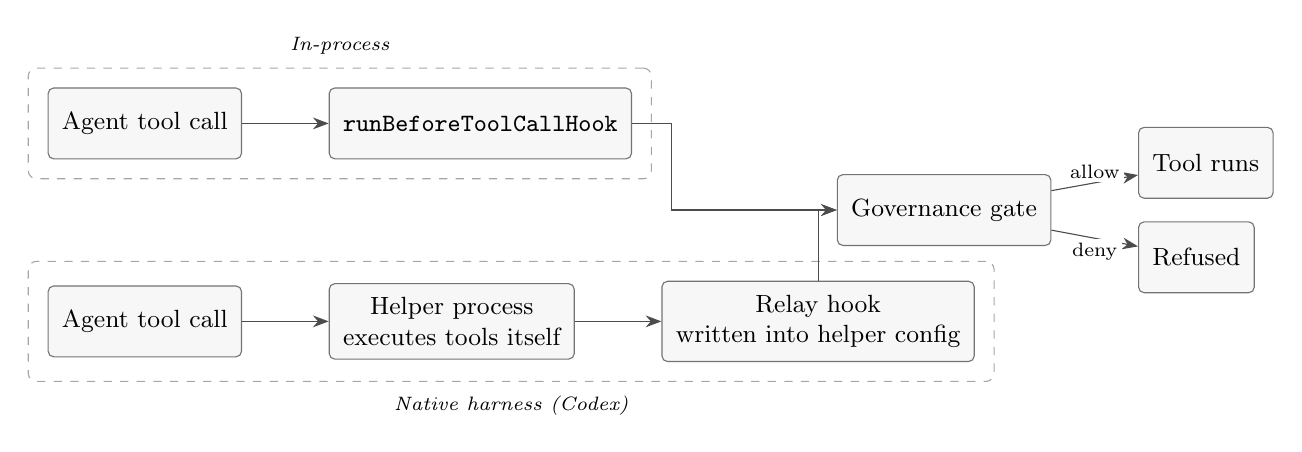
\begin{tikzpicture}[node distance=7mm and 11mm]
  \node[gbox] (a1) {Agent tool call};
  \node[gbox, right=of a1] (h1) {\texttt{runBeforeToolCallHook}};

  \node[gbox, below=16mm of a1] (a2) {Agent tool call};
  \node[gbox, right=of a2] (help) {Helper process\\executes tools itself};
  \node[gbox, right=of help] (relay) {Relay hook\\written into helper config};

  \node[gbox, right=26mm of h1, yshift=-11mm] (gate) {Governance gate};
  \node[gbox, right=of gate, yshift=6mm]  (ok) {Tool runs};
  \node[gbox, right=of gate, yshift=-6mm] (no) {Refused};

  \draw[gflow] (a1) -- (h1);
  \draw[gflow] (a2) -- (help);
  \draw[gflow] (help) -- (relay);
  \draw[gflow] (h1.east) -- ++(5mm,0) |- (gate.west);
  % Up out of the relay, then into the gate's west side. Going right first put the
  % turn to the right of gate.west, so the line was drawn back through the gate and
  % struck out its label (found by looking, 2026-09-20).
  \draw[gflow] (relay.north) |- (gate.west);
  \draw[gflow] (gate) -- node[glab, above] {allow} (ok);
  \draw[gflow] (gate) -- node[glab, below] {deny}  (no);

  \begin{scope}[on background layer]
    \node[ggroup, fit=(a1)(h1)] (g1) {};
    \node[ggroup, fit=(a2)(help)(relay)] (g2) {};
  \end{scope}
  \node[gnote, above=0.5mm of g1] {In-process};
  \node[gnote, below=0.5mm of g2] {Native harness (Codex)};
\end{tikzpicture}
\caption{Two arrangements, one gate. The lower path is governed only if the relay
hook is installed, which on a governed installation it now always is.}
\label{fig:twopaths}
\end{figure}
\end{center}
\clearpage
\subsection*{Figure 3.7 \textnormal{(F11: The check-then-open window)}}
\begin{center}
\begin{figure}[htbp]
\centering
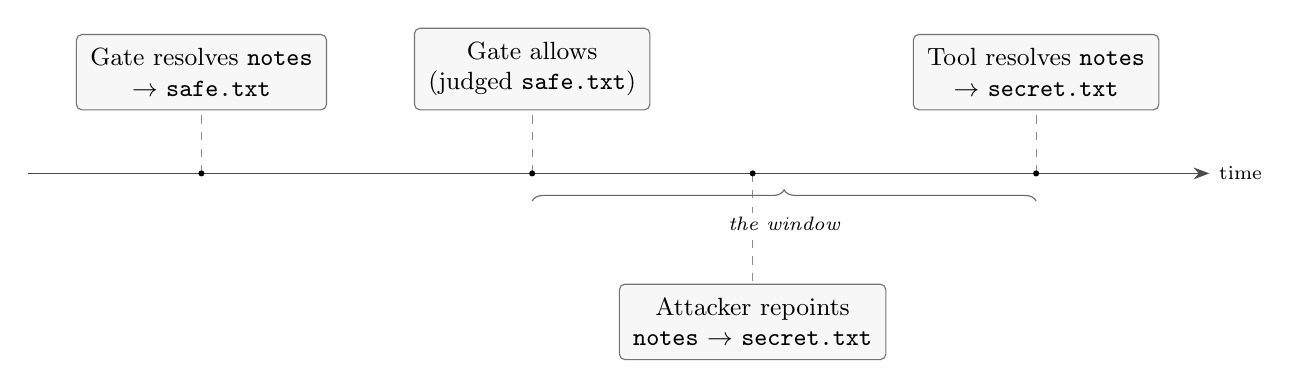
\begin{tikzpicture}[xscale=1.0]
  \draw[gflow] (0,0) -- (15,0) node[right, font=\scriptsize] {time};

  % Positioning is taken off declared coordinates: "of {(x,y)}" typesets its own
  % closing bracket in nullfont and silently drops it (found by compiling, 2026-09-20).
  % The marks were 1.6/4.3/6.0/8.6 apart, which is narrower than the boxes hung off
  % them: the first two boxes overlapped and "Gate resolves notes" lost its last two
  % letters behind the second box (found by looking, 2026-09-20).
  \coordinate (m1) at (2.2,0);
  \coordinate (m2) at (6.4,0);
  \coordinate (m3) at (9.2,0);
  \coordinate (m4) at (12.8,0);

  \node[gbox, above=8mm of m1]  (g)  {Gate resolves \texttt{notes}\\$\rightarrow$ \texttt{safe.txt}};
  \node[gbox, above=8mm of m2]  (a)  {Gate allows\\(judged \texttt{safe.txt})};
  % 14mm, not 8: the brace's label sits in the gap, and at 8mm the box struck it out.
  \node[gbox, below=14mm of m3] (x)  {Attacker repoints\\\texttt{notes} $\rightarrow$ \texttt{secret.txt}};
  \node[gbox, above=8mm of m4]  (t)  {Tool resolves \texttt{notes}\\$\rightarrow$ \texttt{secret.txt}};

  \foreach \p in {2.2, 6.4, 12.8} { \draw[glife] (\p,0) -- (\p,0.8); }
  \draw[glife] (9.2,0) -- (9.2,-1.4);
  \foreach \p in {2.2, 6.4, 9.2, 12.8} { \fill (\p,0) circle (1.1pt); }

  \draw[decorate, decoration={brace, amplitude=4pt}, draw=black!60]
    (6.4,-0.35) -- (12.8,-0.35)
    node[midway, below=4pt, font=\scriptsize\itshape, fill=white, inner sep=1.5pt] {the window};
\end{tikzpicture}
\caption{The check-then-open window. Both resolutions are correct; the defect is
that there are two of them.}
\label{fig:toctou}
\end{figure}
\end{center}
\clearpage
\subsection*{Figure 3.8 \textnormal{(F19: The tenant model)}}
\begin{center}
\begin{figure}[htbp]
\centering
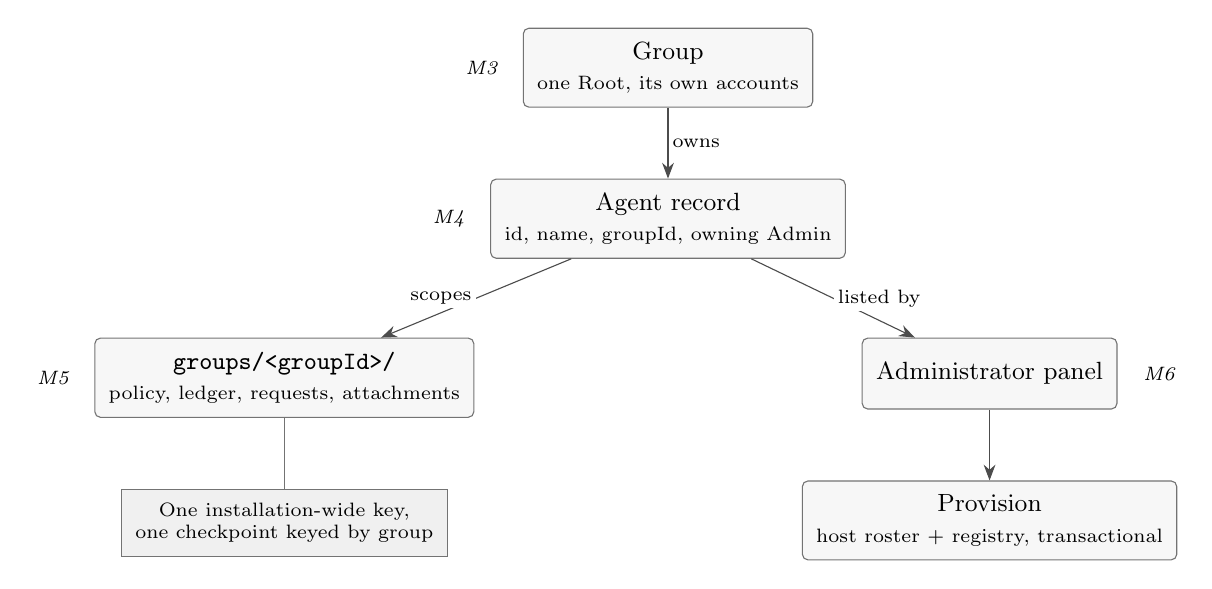
\begin{tikzpicture}[node distance=9mm and 12mm]
  \node[gbox] (g) {Group\\\scriptsize one Root, its own accounts};
  \node[gbox, below=of g] (a) {Agent record\\\scriptsize id, name, groupId, owning Admin};
  \node[gbox, below left=10mm and 2mm of a]  (s) {\texttt{groups/<groupId>/}\\\scriptsize policy, ledger, requests, attachments};
  \node[gbox, below right=10mm and 2mm of a] (ui) {Administrator panel};
  \node[gstore, below=of s]  (k) {One installation-wide key,\\one checkpoint keyed by group};
  \node[gbox,  below=of ui]  (p) {Provision\\\scriptsize host roster + registry, transactional};

  \draw[gflow] (g)  -- node[glab, right] {owns} (a);
  \draw[gflow] (a)  -- node[glab, left]  {scopes} (s);
  \draw[gflow] (a)  -- node[glab, right] {listed by} (ui);
  \draw[gflow] (ui) -- (p);
  \draw[draw=black!55] (s) -- (k);

  \node[gnote, left=2mm of g]  {M3};
  \node[gnote, left=2mm of a]  {M4};
  \node[gnote, left=2mm of s]  {M5};
  \node[gnote, right=2mm of ui] {M6};
\end{tikzpicture}
\caption{The tenant model. Each subtask supplies a noun the next one needs.}
\label{fig:tenant}
\end{figure}
\end{center}
\clearpage
\subsection*{Figure 3.9 \textnormal{(F21: The two-layer Codex permission)}}
\begin{center}
\begin{figure}[htbp]
\centering
  % Measured too wide for the text block when compiled (2026-09-20), so it is
  % scaled to the text width rather than having its font sizes changed.
\resizebox{\textwidth}{!}{%
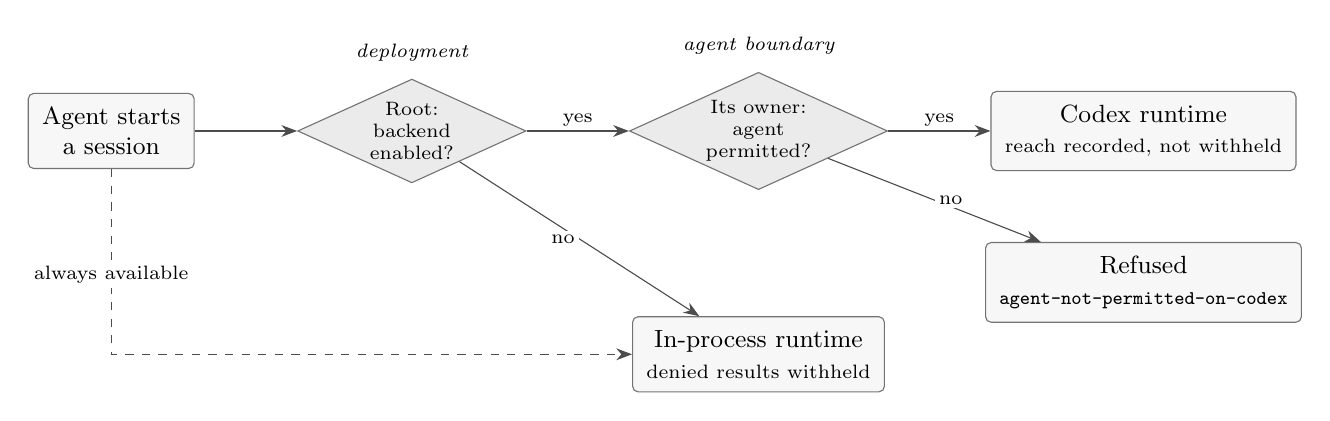
\begin{tikzpicture}[node distance=8mm and 13mm]
  \node[gbox] (a) {Agent starts\\a session};
  \node[gdec, right=of a]  (r)  {Root:\\backend\\enabled?};
  \node[gdec, right=of r]  (ad) {Its owner:\\agent\\permitted?};
  \node[gbox, right=of ad] (cx) {Codex runtime\\\scriptsize reach recorded, not withheld};
  \node[gbox, below=16mm of ad] (ip) {In-process runtime\\\scriptsize denied results withheld};
  \node[gbox, below=9mm of cx]  (ref) {Refused\\\scriptsize \texttt{agent-not-permitted-on-codex}};

  \draw[gflow] (a)  -- (r);
  \draw[gflow] (r)  -- node[glab, above] {yes} (ad);
  \draw[gflow] (ad) -- node[glab, above] {yes} (cx);
  \draw[gflow] (r)  -- node[glab, left]  {no}  (ip);
  \draw[gflow] (ad) -- node[glab, right] {no}  (ref);
  \draw[gdash] (a.south) |- node[glab, below, pos=0.25] {always available} (ip.west);

  \node[gnote, above=1mm of r]  {deployment};
  \node[gnote, above=1mm of ad] {agent boundary};
\end{tikzpicture}}
\caption{The two-layer Codex permission. Both gates must be open; the in-process
runtime needs neither. The second gate is set by the Administrator who owns the
agent, or by Root.}
\label{fig:codexgates}
\end{figure}
\end{center}
\clearpage
\subsection*{Figure 3.10 \textnormal{(F22: Grant a folder, except\dots  (added 2026-09-01))}}
\begin{center}
\begin{figure}[htbp]
\centering
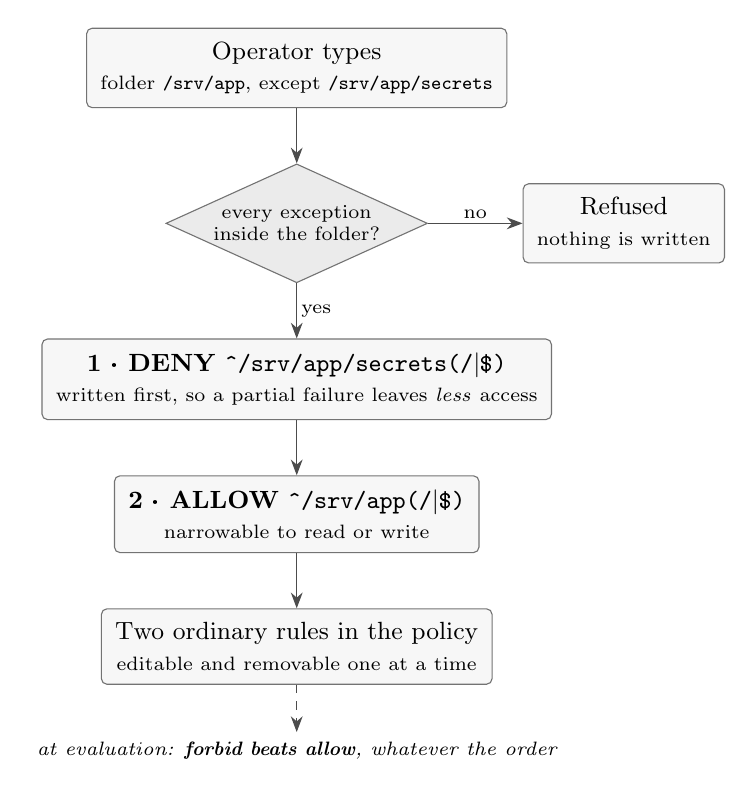
\begin{tikzpicture}[node distance=7mm and 12mm]
  \node[gbox] (in) {Operator types\\\scriptsize folder \texttt{/srv/app}, except \texttt{/srv/app/secrets}};
  \node[gdec, below=of in] (chk) {every exception\\inside the folder?};
  \node[gbox, right=of chk] (ref) {Refused\\\scriptsize nothing is written};
  \node[gbox, below=of chk] (d) {\textbf{1 · DENY} \texttt{\^{}/srv/app/secrets(/\textbar\$)}\\\scriptsize written first, so a partial failure leaves \emph{less} access};
  \node[gbox, below=of d]   (a) {\textbf{2 · ALLOW} \texttt{\^{}/srv/app(/\textbar\$)}\\\scriptsize narrowable to read or write};
  \node[gbox, below=of a]   (out) {Two ordinary rules in the policy\\\scriptsize editable and removable one at a time};
  \node[gnote, below=6mm of out] (gate) {at evaluation: \textbf{forbid beats allow}, whatever the order};

  \draw[gflow] (in)  -- (chk);
  \draw[gflow] (chk) -- node[glab, above] {no} (ref);
  \draw[gflow] (chk) -- node[glab, right] {yes} (d);
  \draw[gflow] (d)   -- (a);
  \draw[gflow] (a)   -- (out);
  \draw[gdash] (out) -- (gate);
\end{tikzpicture}
\caption{A folder grant writes one allow and one deny per exception, denials
first. The exception carves a hole in the grant because forbid beats allow
independently of order.}
\label{fig:foldergrant}
\end{figure}
\end{center}
\clearpage
\subsection*{Figure 3.11 \textnormal{(F23: ``Always allow'', an approval that finishes after its card has closed (added 2026-09-11))}}
\begin{center}
\begin{figure}[htbp]
\centering
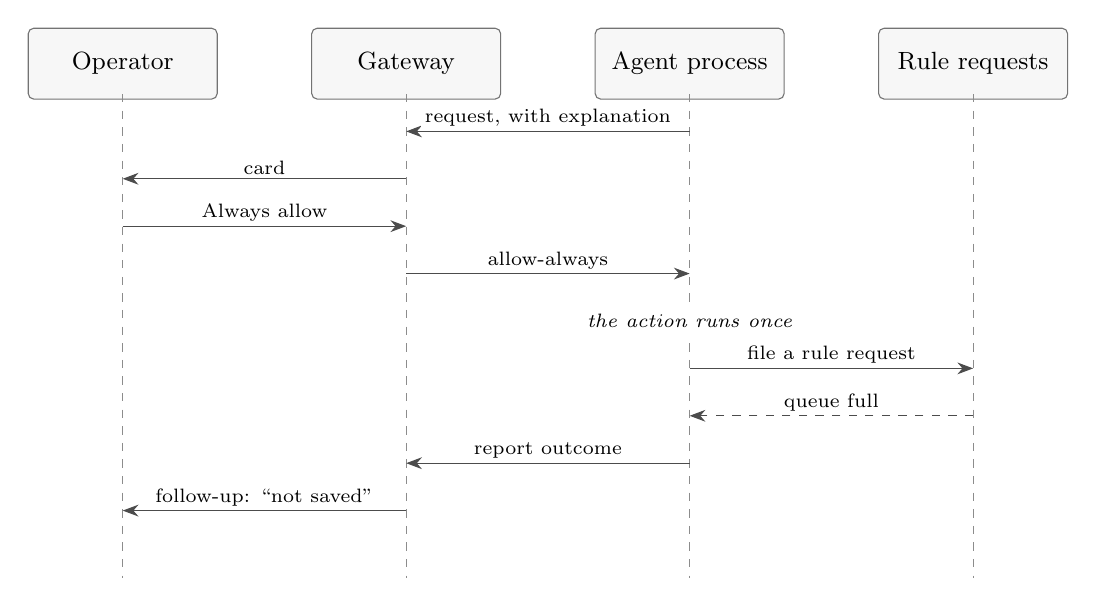
\begin{tikzpicture}[yscale=0.86]
  \foreach \x/\n in {0/{Operator}, 3.6/{Gateway}, 7.2/{Agent process}, 10.8/{Rule requests}} {
    \node[gbox, minimum width=24mm] at (\x,0) {\n};
    \draw[glife] (\x,-0.45) -- (\x,-7.6);
  }
  \draw[gflow] (7.2,-1.0) -- node[glab,above] {request, with explanation} (3.6,-1.0);
  \draw[gflow] (3.6,-1.7) -- node[glab,above] {card} (0,-1.7);
  \draw[gflow] (0,-2.4)   -- node[glab,above] {Always allow} (3.6,-2.4);
  \draw[gflow] (3.6,-3.1) -- node[glab,above] {allow-always} (7.2,-3.1);
  % Filled, so the lifeline it crosses does not run through the words.
  \node[gnote, fill=white] at (7.2,-3.8) {the action runs once};
  \draw[gflow] (7.2,-4.5) -- node[glab,above] {file a rule request} (10.8,-4.5);
  \draw[gdash] (10.8,-5.2) -- node[glab,above] {queue full} (7.2,-5.2);
  \draw[gflow] (7.2,-5.9) -- node[glab,above] {report outcome} (3.6,-5.9);
  \draw[gflow] (3.6,-6.6) -- node[glab,above] {follow-up: ``not saved''} (0,-6.6);
\end{tikzpicture}
\caption{``Always allow'': the operator answers before the rule request exists.
The action runs once, and the request is filed afterwards in the agent's process;
when the organisation's queue (40 requests plus 20 per account) is full, the
outcome travels back through the Gateway as a follow-up. Drawn for a chat run,
whose operator is the Control UI; for a dashboard prompt the card and follow-up
appear on the governance page, to the accounts that manage the agent.}
\label{fig:alwaysallow}
\end{figure}
\end{center}
\clearpage
\subsection*{Figure 3.12 \textnormal{(F24: A task's row and its slot (added 2026-09-11))}}
\begin{center}
\begin{figure}[htbp]
\centering
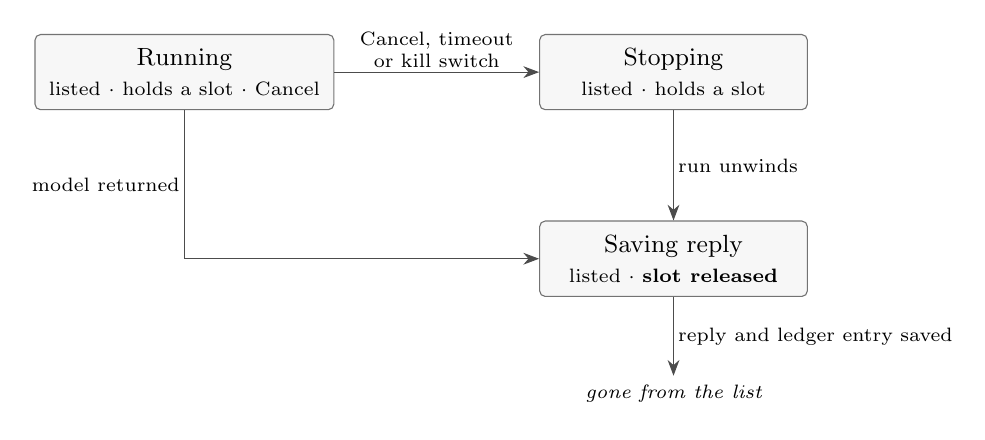
\begin{tikzpicture}[node distance=10mm and 26mm]
  \node[gbox, minimum width=34mm] (run)  {Running\\\scriptsize listed $\cdot$ holds a slot $\cdot$ Cancel};
  \node[gbox, minimum width=34mm, right=of run] (stop) {Stopping\\\scriptsize listed $\cdot$ holds a slot};
  \node[gbox, minimum width=34mm, below=14mm of stop] (save) {Saving reply\\\scriptsize listed $\cdot$ \textbf{slot released}};
  \node[gnote, below=of save] (gone) {gone from the list};
  % Two lines: on one it was wider than the 26mm gap and overlapped both boxes
  % (found by looking, 2026-09-20).
  \draw[gflow] (run)  -- node[glab, above, align=center] {Cancel, timeout\\or kill switch} (stop);
  \draw[gflow] (stop) -- node[glab, right] {run unwinds} (save);
  \draw[gflow] (run)  |- node[glab, pos=0.25, left] {model returned} (save);
  \draw[gflow] (save) -- node[glab, right] {reply and ledger entry saved} (gone);
\end{tikzpicture}
\caption{A task's row and its slot. The row stays listed until the reply is saved,
so a reopened page can recover it; the slot, which alone bounds concurrency, is
released as soon as the task stops executing.}
\label{fig:taskslot}
\end{figure}
\end{center}
\clearpage
\section*{Chapter 4}
\subsection*{Figure 4.1 \textnormal{(F14: Tool coverage, before and after)}}
\begin{center}
\begin{figure}[htbp]
\centering
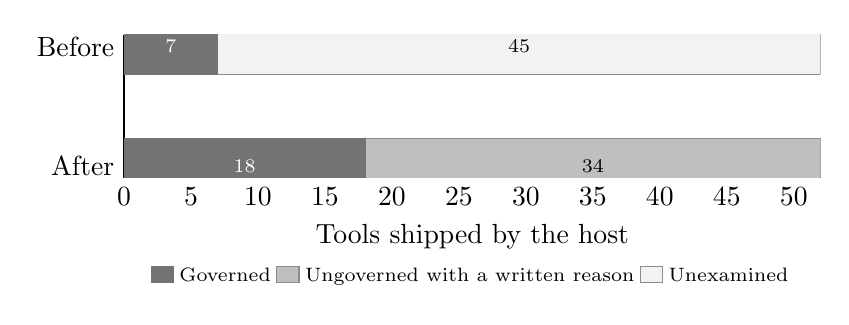
\begin{tikzpicture}
\begin{axis}[
  xbar stacked, width=0.86\textwidth, height=34mm,
  xmin=0, xmax=52, bar width=7mm,
  ytick=data, symbolic y coords={After, Before},
  axis lines*=left, tick style={draw=none},
  xlabel={Tools shipped by the host},
  legend style={at={(0.5,-0.55)}, anchor=north, legend columns=3, draw=none,
                font=\scriptsize},
  % "\addplot+" takes pgfplots' default cycle, which colours the value labels
  % blue, red and brown. This file is greyscale by design, so the plots are set
  % explicitly and the labels are told what colour to be (found by looking,
  % 2026-09-20). Explicit symbolic meta lets a zero segment carry no label.
  every node near coord/.append style={font=\scriptsize, text=black},
  point meta=explicit symbolic,
]
  \addplot[fill=black!55, draw=black!55, nodes near coords,
           every node near coord/.append style={text=white}]
    coordinates {(7,Before) [7] (18,After) [18]};
  \addplot[fill=black!25, draw=black!45, nodes near coords]
    coordinates {(0,Before) [] (34,After) [34]};
  \addplot[fill=black!5,  draw=black!45, nodes near coords]
    coordinates {(45,Before) [45] (0,After) []};
  \legend{Governed, Ungoverned with a written reason, Unexamined}
\end{axis}
\end{tikzpicture}
\caption{Tool coverage before and after. Both bars are the same length, because the
host ships the same fifty-two tools either way; what changed is their composition.
The governed share went from seven to eighteen, and, more to the point, the part
that is not governed stopped being an unexamined gap and became thirty-four
decisions each with a written reason.}
\label{fig:coverage}
\end{figure}
\end{center}
\clearpage
\subsection*{Figure 4.2 \textnormal{(F17: Defects by the age of the code containing them)}}
\begin{center}
\begin{figure}[htbp]
\centering
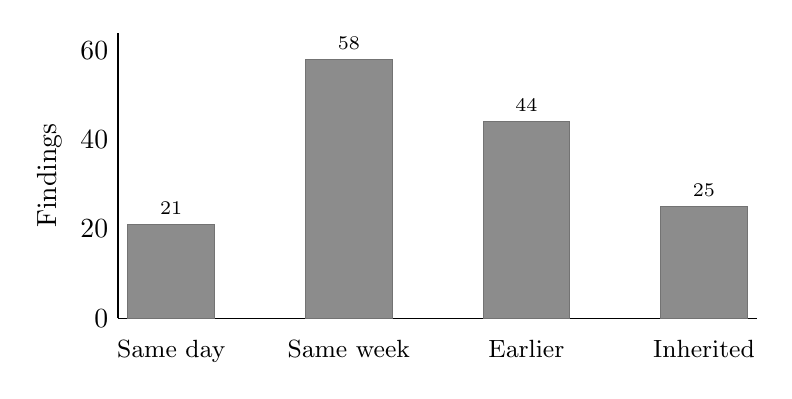
\begin{tikzpicture}
\begin{axis}[
  ybar, width=0.8\textwidth, height=52mm,
  ymin=0, bar width=11mm,
  symbolic x coords={Same day, Same week, Earlier, Inherited},
  xtick=data, axis lines*=left, tick style={draw=none},
  ylabel={Findings}, nodes near coords,
  % text=black: "\addplot+" would take pgfplots' cycle and colour the labels blue,
  % and this file is greyscale by design (found by looking, 2026-09-20).
  every node near coord/.append style={font=\scriptsize, text=black},
  x tick label style={font=\small},
]
  % PLACEHOLDER VALUES. These four numbers sum to 148, the finding total when
  % they were written (376 on 2026-09-19), and the split between the buckets
  % was NEVER measured. Recommended cut; see the state note above.
  \addplot[fill=black!45, draw=black!55]
    coordinates {(Same day,21) (Same week,58) (Earlier,44) (Inherited,25)};
\end{axis}
\end{tikzpicture}
\caption{\textbf{Placeholder values, not measured.} Defects by the age of the code
containing them. The four bars sum to 148, the finding total when they were
written, and the split between the buckets has never been derived from the
register. The shape is the argument (the distribution does not favour old code,
which is why reviewing continuously beats reviewing once) but the numbers must be
re-derived before this figure goes into the report.}
\label{fig:defectage}
\end{figure}
\end{center}
\clearpage
\end{document}
